\appendix

\newpage
\phantomsection
\section*{Appendix}
\addcontentsline{toc}{section}{Appendix}

%====================================================
% A.1 Rankable and Unrankable Pairs
%====================================================

\phantomsection
\subsection*{A.1 Rankable and Unrankable Brother Pairs}
\addcontentsline{toc}{subsection}{A.1 Rankable and Unrankable Brother Pairs}

\begin{figure}[H]
\centering
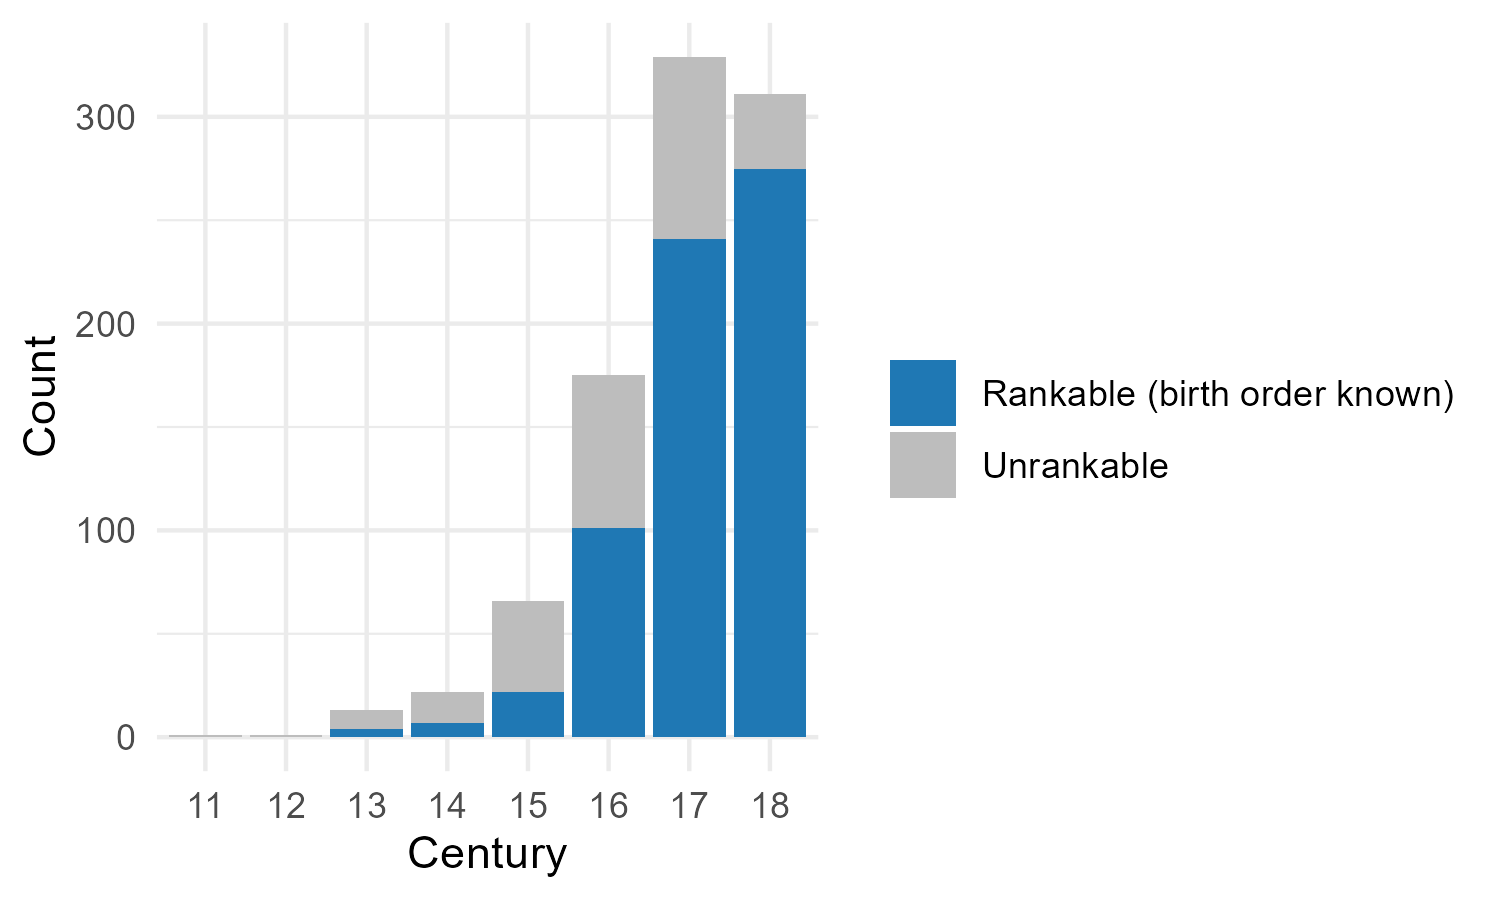
\includegraphics[width=0.72\textwidth]{figures/Plot_Rankable_vs_Unrankable.png}

\caption{Rankable and Unrankable Brother Pairs Across Time}
\label{fig:rankable_unrankable}

\vspace{4pt}
\begin{minipage}{\textwidth}
\footnotesize
\textit{Notes:} The figure shows the distribution of rankable and unrankable brother pairs across centuries. Rankable pairs are those for which birth order can be identified using year-of-birth information.
\end{minipage}

\end{figure}

\FloatBarrier

\begin{table}[H]
\centering
\caption{Comparison Between Rankable and Unrankable Brother Pairs}
\label{tab:rankable_compare}

\begin{tablebody}
\begin{tabular}{l c c}
\toprule
 & \textbf{Rankable} & \textbf{Unrankable} \\
\midrule
Brother pairs & 645 & 268 \\
Mean age gap & 7.22 & -- \\
Mean entry age & 29.43 & 27.06 \\
Father in academia (share) & 0.388 & 0.410 \\
Mean titles & 10.84 & 1.87 \\
Share individuals with no titles & 0.402 & 0.816 \\
Share pairs with no titles & 0.254 & 0.693 \\
\bottomrule
\end{tabular}
\end{tablebody}

\vspace{4pt}
\begin{minipage}{\textwidth}
\footnotesize
\textit{Notes:} The table compares rankable and unrankable brother pairs. Rankable pairs are those for which birth order can be identified using year-of-birth information.
\end{minipage}

\end{table}

\FloatBarrier

%====================================================
% A.2 Entry into Academia and Age Gaps
%====================================================

\phantomsection
\subsection*{A.2 Entry into Academia and Age Gaps}
\addcontentsline{toc}{subsection}{A.2 Entry into Academia and Age Gaps}

\begin{figure}[H]
\centering
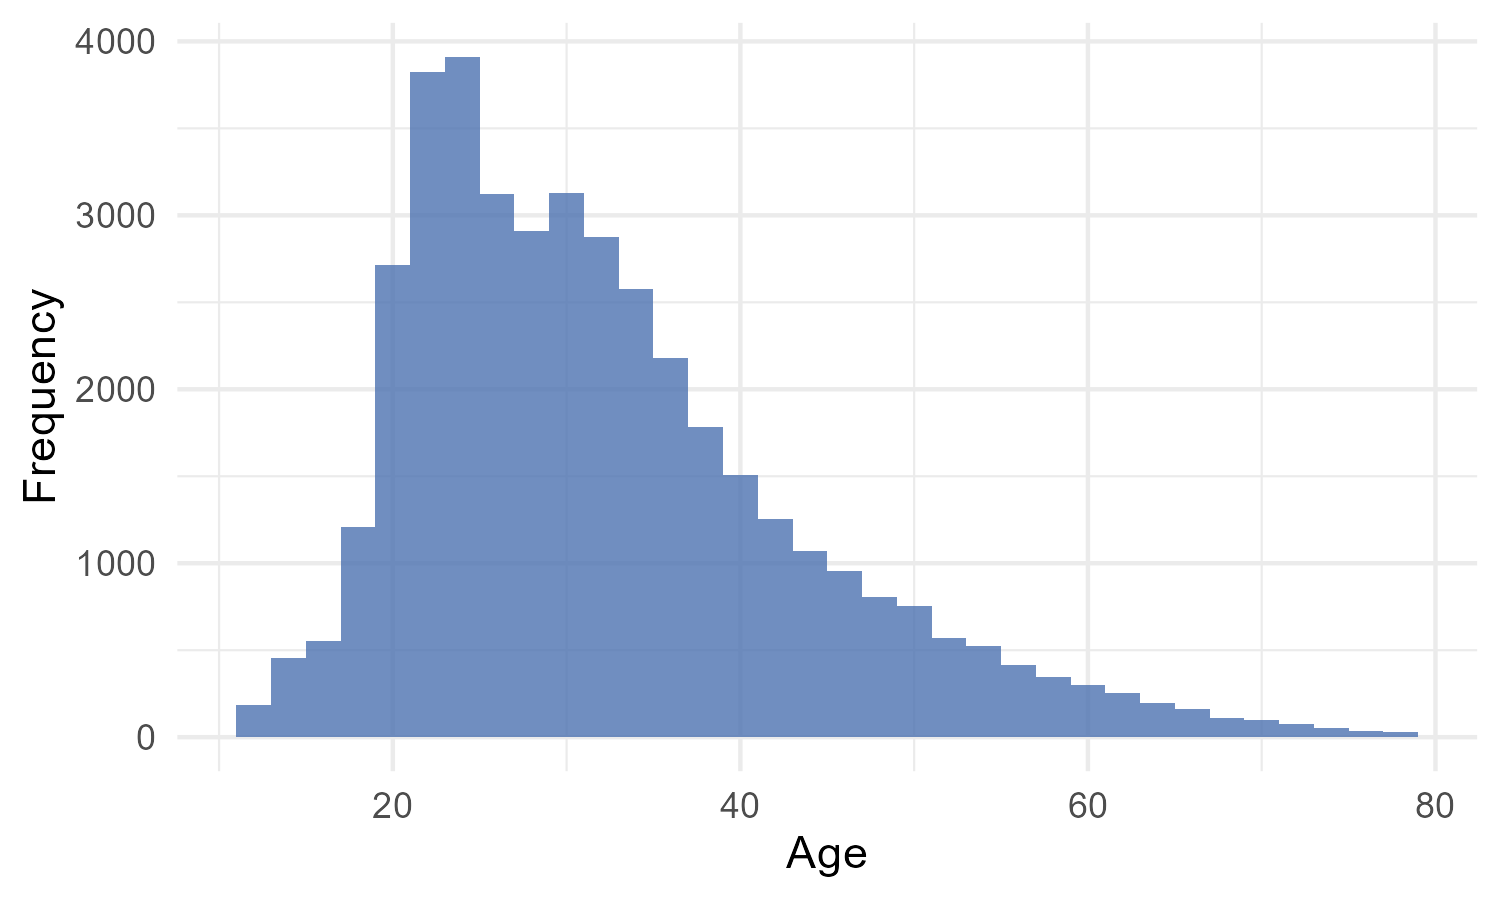
\includegraphics[width=0.68\textwidth]{figures/Plot_Age_Entry.png}

\caption{Distribution of Age at Entry into Academia}
\label{fig:age_entry}

\vspace{4pt}
\begin{minipage}{\textwidth}
\footnotesize
\textit{Notes:} The figure presents the distribution of age at first recorded academic activity for scholars with available information on both birth year and academic activity. Age at entry is computed as the difference between the first recorded academic year and the year of birth.
\end{minipage}

\end{figure}

\FloatBarrier

\begin{figure}[H]
\centering
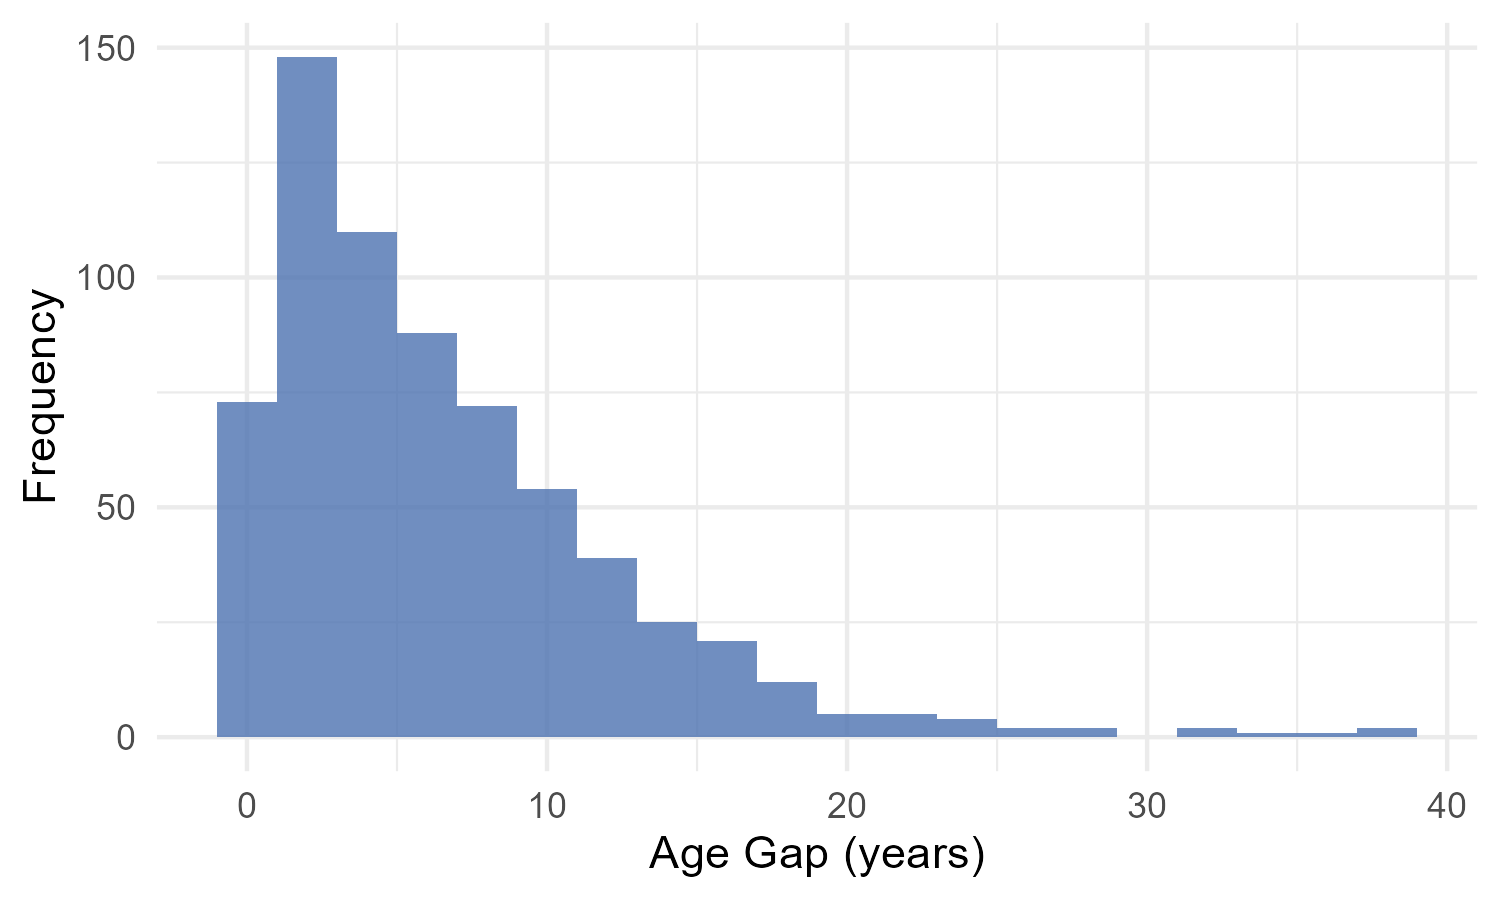
\includegraphics[width=0.68\textwidth]{figures/Plot_Age_Gap_Histogram.png}

\caption{Distribution of Age Gaps Between Brothers}
\label{fig:age_gap}

\vspace{4pt}
\begin{minipage}{\textwidth}
\footnotesize
\textit{Notes:} The histogram displays the distribution of age differences between older and younger brothers in rankable pairs.
\end{minipage}

\end{figure}

\FloatBarrier


%====================================================
% A.3 Historical Productivity Patterns
%====================================================

\phantomsection
\subsection*{A.3 Historical Productivity Patterns}
\addcontentsline{toc}{subsection}{A.3 Historical Productivity Patterns}

\begin{figure}[H]
\centering
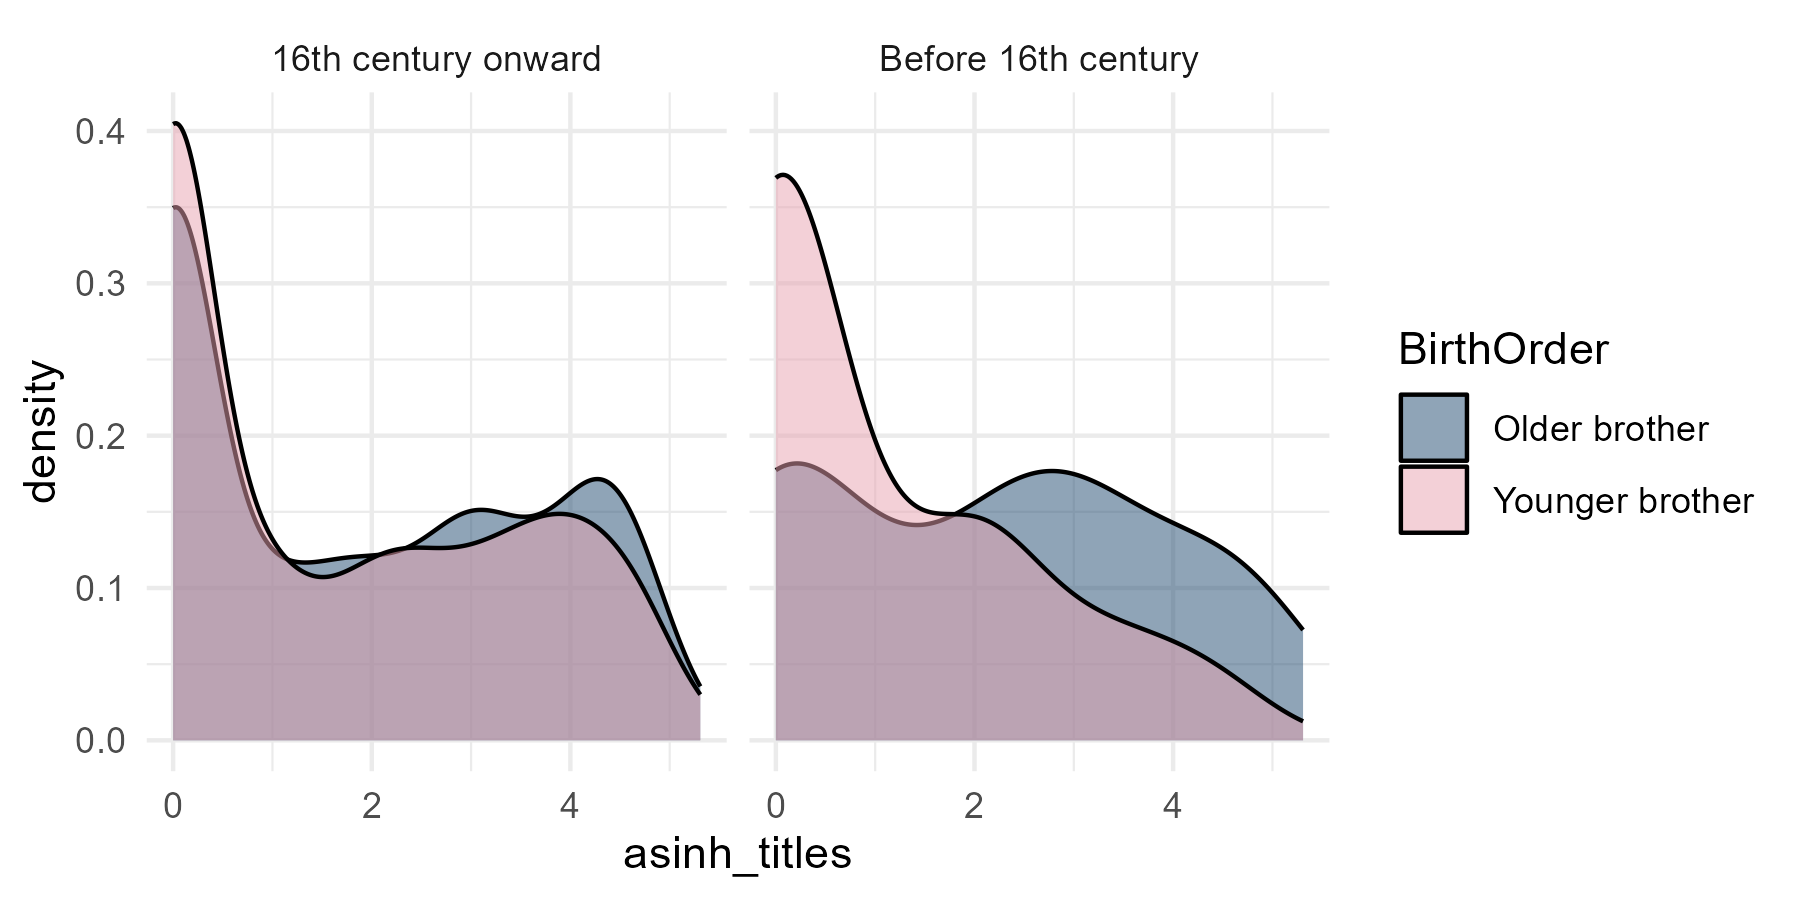
\includegraphics[width=0.72\textwidth]{figures/Plot_Productivity_Distribution_Period.png}

\caption{Distribution of Scholarly Productivity Across Historical Periods}
\label{fig:productivity_period}

\vspace{4pt}
\begin{minipage}{\textwidth}
\footnotesize
\textit{Notes:} The figure compares the distribution of asinh-transformed scholarly productivity before and after the sixteenth century.
\end{minipage}

\end{figure}

\FloatBarrier

\begin{figure}[H]
\centering
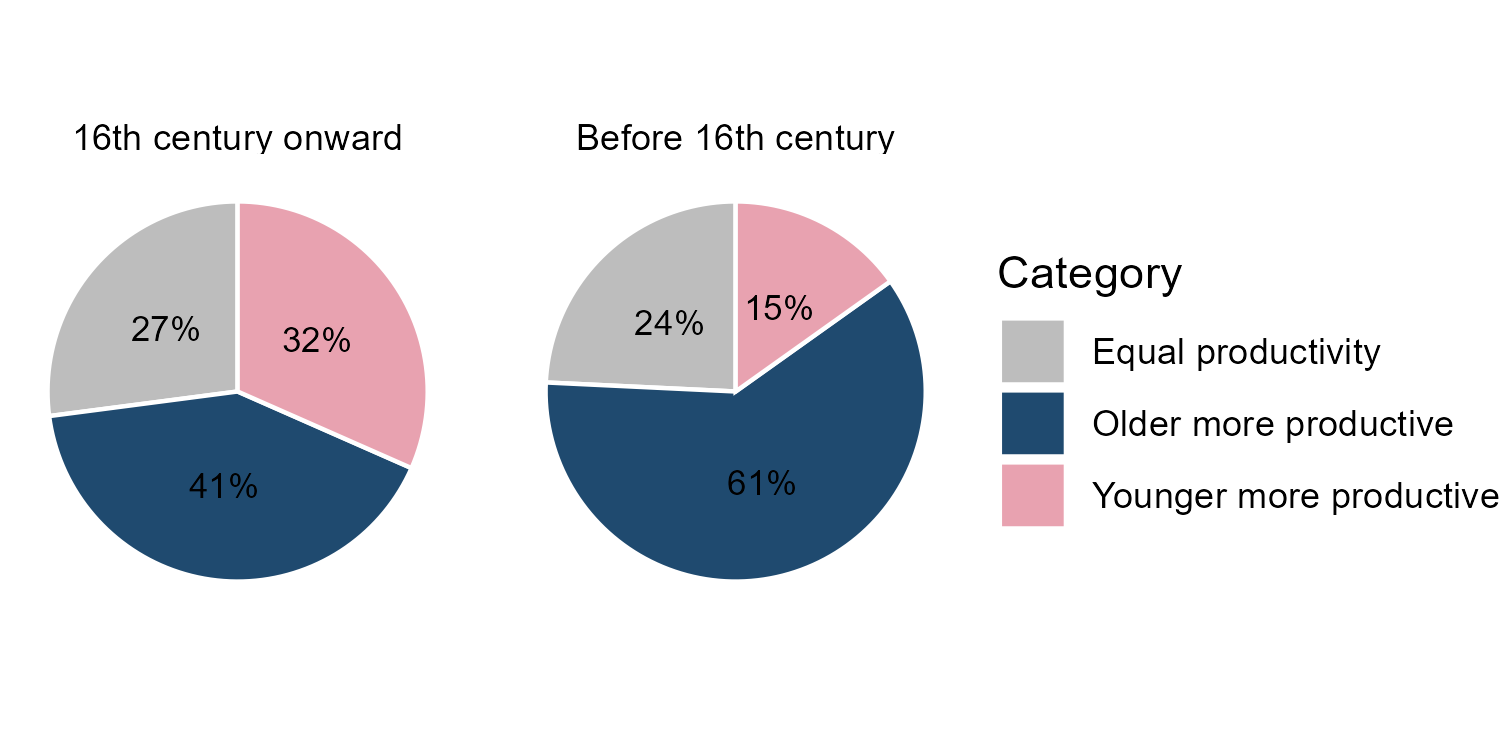
\includegraphics[width=0.68\textwidth]{figures/Pie_Productivity_Period.png}

\caption{Birth-Order Productivity Comparisons by Historical Period}
\label{fig:birthorder_period}

\vspace{4pt}
\begin{minipage}{\textwidth}
\footnotesize
\textit{Notes:} The figure compares the proportion of pairs in which older brothers, younger brothers, or neither sibling exhibit higher productivity across historical periods.
\end{minipage}

\end{figure}

\FloatBarrier

\begin{table}[H]
\centering
\caption{Birth-Order Differences Before and After the 16th Century}
\label{tab:prepost16}

\begin{tablebody}
\begin{tabular}{l c c}
\toprule
 & \textbf{Before 16th century} & \textbf{16th century onward} \\
\midrule
Brother pairs & 33 & 612 \\
Mean age gap & 10.18 & 7.06 \\
Mean titles (older brothers) & 13.94 & 11.78 \\
Mean titles (younger brothers) & 4.45 & 10.08 \\
Older brother more productive (share) & 0.606 & 0.405 \\
Pairs with no titles (share) & 0.242 & 0.255 \\
Father in academia (share) & 0.303 & 0.392 \\
\bottomrule
\end{tabular}
\end{tablebody}

\vspace{4pt}
\begin{minipage}{\textwidth}
\footnotesize
\textit{Notes:} Descriptive statistics for the sample of rankable brother pairs, i.e. pairs for which birth order can be identified, reported separately for observations before and after the sixteenth century. Scholarly productivity is measured using the number of titles recorded in VIAF. Shares are reported as proportions.
\end{minipage}

\end{table}

\FloatBarrier

\begin{table}[H]
\centering
\caption{Paired Comparisons by Historical Period}
\label{tab:period_ttests}

\begin{tablebody}
\begin{tabular}{l c c c}
\toprule
\textbf{Period} & \textbf{Mean Difference} & \textbf{p-value} & \textbf{N} \\
\midrule

Before 16th century
& 1.046*** & 0.0007 & 33 \\

16th century onward
& 0.202*** & 0.0063 & 612 \\

\bottomrule
\end{tabular}
\end{tablebody}

\vspace{4pt}
\begin{minipage}{\textwidth}
\footnotesize
\textit{Notes:} The table reports paired comparisons of the inverse hyperbolic sine (asinh) difference in titles between older and younger brothers across broad historical periods. Mean differences are calculated as older minus younger. \textit{Significance levels:} *** $p<0.01$, ** $p<0.05$, * $p<0.10$.
\end{minipage}

\end{table}

\FloatBarrier

%====================================================
% A.4 Inheritance Systems and Historical Composition
%====================================================

\phantomsection
\subsection*{A.4 Inheritance Systems and Historical Composition}
\addcontentsline{toc}{subsection}{A.4 Inheritance Systems and Historical Composition}

\begin{table}[H]
\centering
\caption{Inheritance Systems in the Sample}
\label{tab:inheritance_composition}

\begin{tablebody}
\begin{tabular}{l c c}
\toprule
\textbf{Inheritance system} & \textbf{Count} & \textbf{Share} \\
\midrule
Egalitarian & 194 & 0.301 \\
Non-egalitarian & 300 & 0.465 \\
Unknown & 151 & 0.234 \\
\bottomrule
\end{tabular}
\end{tablebody}

\vspace{4pt}
\begin{minipage}{\textwidth}
\footnotesize
\textit{Notes:} Inheritance systems are assigned using Todd's classification at the NUTS3 level. Shares are computed over the full analytical sample.
\end{minipage}

\end{table}
\FloatBarrier

%====================================================
% A.5 Additional Institutional Interaction Specifications
%====================================================

\phantomsection
\subsection*{A.5 Additional Institutional Interaction Specifications}
\addcontentsline{toc}{subsection}{A.5 Additional Institutional Interaction Specifications}

\begin{table}[H]
\centering
\caption{Inheritance Systems and Birth-Order Productivity After the Sixteenth Century}
\label{tab:inheritance_post15}

\begin{tablebody}
\begin{tabular}{l c}
\toprule
 & (1) \\
 & \textit{Asinh difference in titles} \\
\midrule

Intercept
& 0.998*** \\
& (0.305) \\

Non-egalitarian inheritance
& -0.362 \\
& (0.631) \\

Inheritance unknown
& -1.716 \\
& (1.258) \\

Post-16th century
& -1.134*** \\
& (0.314) \\

Age gap
& 0.019* \\
& (0.010) \\

Father in academia
& -0.178 \\
& (0.149) \\

Different institution
& 0.472*** \\
& (0.180) \\

Non-egalitarian $\times$ Post-16th
& 0.533 \\
& (0.655) \\

Unknown inheritance $\times$ Post-16th
& 1.897 \\
& (1.276) \\

\midrule
Clustered SE (family) & Yes \\
\midrule
Observations & 645 \\
R$^{2}$ & 0.034 \\
Adj. R$^{2}$ & 0.022 \\
\bottomrule
\end{tabular}
\end{tablebody}

\vspace{4pt}
\begin{minipage}{\textwidth}
\footnotesize
\textit{Notes:} The dependent variable is the inverse hyperbolic sine (asinh) of the difference in titles between older and younger brothers. The specification interacts inheritance systems with an indicator for observations from the sixteenth century onward. The split is motivated by the limited variation in inheritance-system classifications observed before the sixteenth century. Standard errors are clustered at the family level. \textit{Significance levels:} *** $p<0.01$, ** $p<0.05$, * $p<0.10$.
\end{minipage}

\end{table}

\FloatBarrier


%====================================================
% A.6 Robustness Checks
%====================================================

\phantomsection
\subsection*{A.6 Robustness Checks}
\addcontentsline{toc}{subsection}{A.6 Robustness Checks}

\begin{table}[H]
\centering
\caption{Alternative Sample Specifications}
\label{tab:robustness}

\begin{tablebody}
\begin{tabular}{l c c}
\toprule
 & (1) & (2) \\
 & \textit{Age gap $\leq 20$} & \textit{Two-son families only} \\
\midrule
 & \multicolumn{2}{c}{\textit{Asinh difference in titles}} \\
\midrule

Constant
& -0.175
& -0.151 \\
& (0.209)
& (0.223) \\

Non-egalitarian inheritance
& 0.153
& 0.047 \\
& (0.179)
& (0.202) \\

Inheritance unknown
& 0.167
& 0.020 \\
& (0.211)
& (0.240) \\

Age gap
& 0.022
& 0.014 \\
& (0.016)
& (0.013) \\

Father in academia
& -0.168
& -0.054 \\
& (0.152)
& (0.177) \\

Different institution
& 0.478*** 
& 0.493** \\
& (0.182)
& (0.202) \\

13th century
& 0.080
& -0.330 \\
& (0.231)
& (0.264) \\

14th century
& 1.761*** 
& 1.687** \\
& (0.550)
& (0.850) \\

15th century
& 0.796** 
& 1.038*** \\
& (0.371)
& (0.387) \\

16th century
& -0.023
& 0.235 \\
& (0.231)
& (0.265) \\

17th century
& 0.079
& 0.192 \\
& (0.164)
& (0.187) \\

\midrule
Century indicators & Yes & Yes \\
Clustered SE (family) & Yes & Yes \\
\midrule

Observations & 624 & 467 \\
R$^{2}$ & 0.033 & 0.036 \\
Adj. R$^{2}$ & 0.018 & 0.014 \\

\bottomrule
\end{tabular}
\end{tablebody}

\vspace{4pt}
\begin{minipage}{\textwidth}
\footnotesize
\textit{Notes:} The dependent variable is the inverse hyperbolic sine (asinh) difference in titles between older and younger brothers. Column (1) restricts the sample to brother pairs with an age gap below or equal to twenty years. Column (2) restricts the sample to families with only two sons. All specifications include century indicator variables, with the eighteenth century used as the omitted reference category. Standard errors are clustered at the family level. Across both robustness specifications, differences in institutional affiliation remain positively associated with larger productivity differences between siblings, while inheritance-system coefficients remain statistically insignificant.

\textit{Significance levels:} *** $p<0.01$, ** $p<0.05$, * $p<0.10$.
\end{minipage}

\end{table}

\FloatBarrier

\begin{table}[H]
\centering
\caption{Alternative Measures of Scholarly Visibility}
\label{tab:alt_measures}

\begin{tablebody}
\begin{tabular}{p{5cm} c c c}
\toprule
 & (1) & (2) & (3) \\
 & \textit{Wikipedia length gap} & \textit{Wikipedia languages gap} & \textit{Publishers gap} \\
\midrule

Constant
& 0.077
& -0.203
& -0.559 \\
& (0.231)
& (0.759)
& (0.627) \\

Non-egalitarian inheritance
& -0.027 
& -0.463 
& 0.164 \\
& (0.197) 
& (0.673) 
& (0.575) \\

Inheritance unknown
& -0.199 
& 0.053 
& 0.110 \\
& (0.225) 
& (0.706) 
& (0.670) \\

Age gap
& 0.016 
& 0.050 
& 0.082** \\
& (0.014) 
& (0.036) 
& (0.033) \\

Father in academia
& -0.344** 
& -0.028 
& -0.600 \\
& (0.157) 
& (0.593) 
& (0.467) \\

Different institution
& 0.148 
& 1.885** 
& 1.550*** \\
& (0.187) 
& (0.818) 
& (0.562) \\

13th century
& 0.812 
& 1.694 
& -4.146 \\
& (0.343) 
& (1.483) 
& (1.392) \\

14th century
& 0.139 
& 6.205*** 
& 7.036*** \\
& (0.951) 
& (1.872) 
& (2.527) \\

15th century
& 0.964*** 
& 1.438 
& 2.390 \\
& (0.526) 
& (1.851) 
& (1.792) \\

16th century
& 0.053 
& 0.170 
& 0.271 \\
& (0.241) 
& (0.787) 
& (0.497) \\

17th century
& 0.237 
& -0.061 
& 0.305 \\
& (0.172) 
& (0.770) 
& (0.310) \\

\midrule
Century indicators & Yes & Yes & Yes \\
Clustered SE (family) & Yes & Yes & Yes \\
\midrule

Observations & 645 & 645 & 645 \\
R$^{2}$ & 0.022 & 0.026 & 0.045 \\
Adj. R$^{2}$ & 0.007 & 0.010 & 0.030 \\
\bottomrule
\end{tabular}
\end{tablebody}

\vspace{4pt}
\begin{minipage}{\textwidth}
\footnotesize
\textit{Notes:} Dependent variables are alternative measures of scholarly visibility differences between older and younger brothers. Column (1) uses the inverse hyperbolic sine (asinh) difference in Wikipedia page length. Column (2) uses the difference in the number of Wikipedia language versions. Column (3) uses the difference in the number of publishers associated with VIAF records. All specifications include century indicator variables, with the eighteenth century used as the omitted reference category. Standard errors are clustered at the family level. The results indicate that institutional divergence between siblings is positively associated with broader differences in scholarly visibility, particularly regarding Wikipedia language coverage and publisher networks.

\textit{Significance levels:} *** $p<0.01$, ** $p<0.05$, * $p<0.10$.
\end{minipage}

\end{table}

\FloatBarrier

\begin{table}[H]
\centering
\caption{Logarithmic Specification}
\label{tab:log_regressions}

\begin{tablebody}
\begin{tabular}{lcccc}
\toprule
& (1) & (2) & (3) & (4) \\
\midrule

Constant
& 0.1177
& 0.0256
& 0.0034
& -0.2192 \\
& (0.1530)
& (0.1781)
& (0.2419)
& (0.2718) \\

Age gap 
& 0.0302** 
& 0.0297* 
& 0.0296* 
& 0.0244 \\
& (0.0153) 
& (0.0154) 
& (0.0155) 
& (0.0157) \\

Father in academia 
&  
& -0.1674 
& -0.1748 
& -0.1424 \\
&  
& (0.2036) 
& (0.2037) 
& (0.2070) \\

Different institution 
&  
& 0.5224** 
& 0.5208** 
& 0.5773** \\
&  
& (0.2427) 
& (0.2429) 
& (0.2429) \\

Non-egalitarian inheritance 
&  
&  
& 0.0640 
& 0.1978 \\
&  
&  
& (0.2328) 
& (0.2417) \\

Unknown inheritance system 
&  
&  
& -0.0163 
& 0.1234 \\
&  
&  
& (0.2692) 
& (0.2799) \\

13th century
& & & & 0.0520 \\
& & & & (0.3011) \\

14th century
& & & & 1.8130*** \\
& & & & (0.5829) \\

15th century
& & & & 1.4065*** \\
& & & & (0.5039) \\

16th century
& & & & 0.0711 \\
& & & & (0.3073) \\

17th century
& & & & 0.1507 \\
& & & & (0.2228) \\

\midrule
Century indicators 
& No 
& No 
& No 
& Yes \\

Clustered SE (family) & Yes & Yes & Yes & Yes \\

\midrule

Observations 
& 645 
& 645 
& 645 
& 645 \\

$R^2$ 
& 0.005 
& 0.015 
& 0.015 
& 0.029 \\

Adj. $R^2$ 
& 0.004 
& 0.010 
& 0.007 
& 0.014 \\

\bottomrule
\end{tabular}
\end{tablebody}

\vspace{4pt}
\begin{minipage}{\textwidth}
\footnotesize
\textit{Notes:} The dependent variable is the logarithmic difference in titles between older and younger brothers, computed as 
$\log(\text{Titles}_{Older} + \varepsilon) - \log(\text{Titles}_{Younger} + \varepsilon)$, 
where $\varepsilon = 0.1$. Positive values indicate higher productivity for the older sibling. Standard errors clustered at the family level are reported in parentheses. Column (4) includes century indicator variables, with the eighteenth century used as the omitted reference category.

\textit{Significance levels:} *** $p<0.01$, ** $p<0.05$, * $p<0.10$.
\end{minipage}

\end{table}
\FloatBarrier

\begin{table}[H]
\centering
\caption{Level Specification}
\label{tab:levels_regressions}

\begin{tablebody}
\begin{tabular}{lcccc}
\toprule
& (1) & (2) & (3) & (4) \\
\midrule

Constant
& 0.6422
& -0.1949
& -0.4523
& -2.3098 \\
& (1.1962)
& (1.3309)
& (1.9141)
& (2.1160) \\

Age gap 
& 0.2013* 
& 0.1964* 
& 0.1980* 
& 0.1909* \\
& (0.1028) 
& (0.1012) 
& (0.1017) 
& (0.1030) \\

Father in academia 
&  
& -1.4100 
& -1.3192 
& -1.0555 \\
&  
& (1.6792) 
& (1.6453) 
& (1.6620) \\

Different institution 
&  
& 4.5978** 
& 4.6302** 
& 5.1599** \\
&  
& (2.0256) 
& (2.0235) 
& (2.0156) \\

Non-egalitarian inheritance 
&  
&  
& -0.2075 
& 0.9186 \\
&  
&  
& (1.8637) 
& (1.9094) \\

Unknown inheritance system 
&  
&  
& 1.2691 
& 2.5016 \\
&  
&  
& (2.1364) 
& (2.1987) \\

13th century
& & & & 0.4273 \\
& & & & (2.1678) \\

14th century
& & & & 27.7798*** \\
& & & & (8.8441) \\

15th century
& & & & 4.7241 \\
& & & & (3.5811) \\

16th century
& & & & -0.0156 \\
& & & & (2.5141) \\

17th century
& & & & 0.9846 \\
& & & & (1.8061) \\

\midrule
Century indicators 
& No 
& No 
& No 
& Yes \\

Clustered SE (family) & Yes & Yes & Yes & Yes \\
\midrule

Observations 
& 645 
& 645 
& 645 
& 645 \\

$R^2$ 
& 0.004 
& 0.016 
& 0.017 
& 0.038 \\

Adj. $R^2$ 
& 0.002 
& 0.011 
& 0.009 
& 0.023 \\

\bottomrule
\end{tabular}
\end{tablebody}

\vspace{4pt}
\begin{minipage}{\textwidth}
\footnotesize
\textit{Notes:} The dependent variable is the level difference in titles between older and younger brothers. Positive values indicate higher productivity for the older sibling. Standard errors clustered at the family level are reported in parentheses. Column (4) includes century indicator variables, with the eighteenth century used as the omitted reference category.

\textit{Significance levels:} *** $p<0.01$, ** $p<0.05$, * $p<0.10$.
\end{minipage}

\end{table}
\FloatBarrier

%====================================================
% APPENDIX TABLE — LOG SPECIFICATION BY PERIOD
%====================================================

\begin{table}[H]
\centering
\caption{Birth-Order Productivity Gap by Historical Period (Log Specification)}
\label{tab:period_log_appendix}

\begin{tablebody}
\begin{tabular}{l c c}
\toprule
& (1) & (2) \\
& Pre-16th century & 16th century onward \\
& \multicolumn{2}{c}{\textit{Log difference in titles}} \\
\midrule

Constant
& -0.450
& -0.170 \\
& (1.009)
& (0.276) \\

Non-egalitarian inheritance
& -0.453
& 0.211 \\
& (0.914)
& (0.248) \\

Unknown inheritance system
& -1.568
& 0.155 \\
& (2.551)
& (0.283) \\

Age gap
& 0.174***
& 0.014 \\
& (0.044)
& (0.016) \\

Father in academia
& 0.829
& -0.144 \\
& (1.084)
& (0.212) \\

Different institution
& 0.620
& 0.587** \\
& (1.021)
& (0.247) \\

Century 13
& -2.386** 
& --- \\
& (0.923)
& --- \\

Century 14
& 1.049
& --- \\
& (0.919)
& --- \\

Century 16
& ---
& 0.082 \\
& ---
& (0.307) \\

Century 17
& ---
& 0.159 \\
& ---
& (0.222) \\

\midrule
Century controls & Yes & Yes \\
Clustered SE (family) & Yes & Yes \\
\midrule
Observations & 33 & 612 \\
R$^{2}$ & 0.341 & 0.015 \\
Adj. R$^{2}$ & 0.156 & 0.004 \\
\bottomrule
\end{tabular}
\end{tablebody}

\vspace{4pt}
\begin{minipage}{\textwidth}
\footnotesize
\textit{Notes:} The dependent variable is the logarithmic difference in titles between older and younger brothers. Positive values indicate higher productivity for the older sibling. All specifications include century controls. The omitted century category is the 15th century in Column (1) and the 18th century in Column (2). Standard errors clustered at the family level are reported in parentheses.

\textit{Significance levels:} *** $p<0.01$, ** $p<0.05$, * $p<0.10$.
\end{minipage}

\end{table}
\FloatBarrier

%====================================================
% APPENDIX TABLE — LEVELS SPECIFICATION BY PERIOD
%====================================================

\begin{table}[H]
\centering
\caption{Birth-Order Productivity Gap by Historical Period (Levels Specification)}
\label{tab:period_levels_appendix}

\begin{tablebody}
\begin{tabular}{l c c}
\toprule
& (1) & (2) \\
& Pre-16th century & 16th century onward \\
& \multicolumn{2}{c}{\textit{Difference in titles}} \\
\midrule

Constant
& -1.246
& -2.478 \\
& (4.768)
& (2.149) \\

Non-egalitarian inheritance
& -12.663**
& 1.447 \\
& (5.064)
& (1.957) \\

Unknown inheritance system
& -20.357
& 3.196 \\
& (16.716)
& (2.218) \\

Age gap
& 0.702**
& 0.168 \\
& (0.333)
& (0.108) \\

Father in academia
& 0.173
& -0.905 \\
& (7.440)
& (1.701) \\

Different institution
& 20.117**
& 4.688** \\
& (8.241)
& (2.044) \\

Century 13
& -11.350
& --- \\
& (7.256)
& --- \\

Century 14
& 23.641**
& --- \\
& (10.286)
& --- \\

Century 16
& ---
& 0.041 \\
& ---
& (2.518) \\

Century 17
& ---
& 0.954 \\
& ---
& (1.803) \\

\midrule
Century controls & Yes & Yes \\
Clustered SE (family) & Yes & Yes \\
\midrule
Observations & 33 & 612 \\
R$^{2}$ & 0.494 & 0.018 \\
Adj. R$^{2}$ & 0.352 & 0.007 \\
\bottomrule
\end{tabular}
\end{tablebody}

\vspace{4pt}
\begin{minipage}{\textwidth}
\footnotesize
\textit{Notes:} The dependent variable is the raw difference in titles between older and younger brothers. Positive values indicate higher productivity for the older sibling. All specifications include century controls. The omitted century category is the 15th century in Column (1) and the 18th century in Column (2). Standard errors clustered at the family level are reported in parentheses.

\textit{Significance levels:} *** $p<0.01$, ** $p<0.05$, * $p<0.10$.
\end{minipage}

\end{table}
\FloatBarrier

\newpage
%====================================================
% APPENDIX TABLE — COUNTRY CONTROLS
%====================================================

\begin{center}

\small

\begin{longtable}{l c}

\caption{Birth-Order Productivity Gap with Country Controls}
\label{tab:country_fe_appendix} \\

\toprule
& (1) \\
& \textit{Asinh difference in titles} \\
\midrule
\endfirsthead

\toprule
& (1) \\
& \textit{Asinh difference in titles} \\
\midrule
\endhead

\midrule
\multicolumn{2}{r}{\textit{Continued on next page}} \\
\midrule
\endfoot

\bottomrule
\endlastfoot

Constant
& -0.149 \\
& (0.348) \\

Non-egalitarian inheritance
& 0.243 \\
& (0.258) \\

Unknown inheritance system
& -0.044 \\
& (0.355) \\

Age gap
& 0.020* \\
& (0.011) \\

Father in academia
& -0.143 \\
& (0.187) \\

Different institution
& 0.388* \\
& (0.200) \\

13th century
& 0.064 \\
& (0.280) \\

14th century
& 1.776*** \\
& (0.577) \\

15th century
& 0.981*** \\
& (0.349) \\

16th century
& 0.092 \\
& (0.224) \\

17th century
& 0.140 \\
& (0.167) \\

\midrule
Country controls (reference: Germany (DEU)) \\
\midrule

Austria (AUT)
& -2.169*** \\
& (0.423) \\

Belgium (BEL)
& 1.691* \\
& (1.021) \\

Belarus (BLR)
& -1.783** \\
& (0.850) \\

Switzerland (CHE)
& -0.172 \\
& (0.461) \\

Denmark (DNK)
& -0.572 \\
& (0.487) \\

Spain (ESP)
& 0.483 \\
& (0.380) \\

Finland (FIN)
& -0.484 \\
& (0.738) \\

France (FRA)
& -0.156 \\
& (0.277) \\

United Kingdom (GBR)
& -0.086 \\
& (0.286) \\

Croatia (HRV)
& 2.341** \\
& (0.983) \\

Ireland (IRL)
& 0.447 \\
& (0.823) \\

Italy (ITA)
& 0.018 \\
& (0.349) \\

Lithuania (LTU)
& 2.226*** \\
& (0.856) \\

Netherlands (NLD)
& 0.034 \\
& (0.371) \\

Norway (NOR)
& 0.164 \\
& (0.278) \\

Poland (POL)
& -0.656 \\
& (0.709) \\

Portugal (PRT)
& -0.676 \\
& (0.899) \\

Russia (RUS)
& 1.061** \\
& (0.511) \\

Slovakia (SVK)
& 1.151*** \\
& (0.342) \\

Sweden (SWE)
& -0.186 \\
& (0.449) \\

Ukraine (UKR)
& 0.445 \\
& (0.693) \\

United States (USA)
& 0.074 \\
& (0.359) \\

Unknown country
& -1.959*** \\
& (0.313) \\

\midrule
Century controls & Yes \\
Country categorical controls & Yes \\
Clustered SE (family) & Yes \\
\midrule
Observations & 645 \\
R$^{2}$ & 0.080 \\
Adj. R$^{2}$ & 0.031 \\

\end{longtable}

\vspace{4pt}

\begin{minipage}{0.95\textwidth}
\footnotesize
\textit{Notes:} The dependent variable is the inverse hyperbolic sine (asinh) difference in titles between older and younger brothers. Positive values indicate higher productivity for the older sibling. The specification includes century indicator variables, with the eighteenth century used as the omitted reference category, together with country categorical controls constructed from the birthplace country identifiers of the brothers. Germany (DEU), the country with the largest number of observations, is used as the omitted reference category. Inheritance systems remain assigned at the regional NUTS level. Several countries contain only a very limited number of observations, reflecting the highly uneven geographical distribution of historically identifiable scholarly brother pairs. Standard errors clustered at the family level are reported in parentheses.

\textit{Significance levels:} *** $p<0.01$, ** $p<0.05$, * $p<0.10$.
\end{minipage}

\end{center}
\FloatBarrier